\section{Training und Hpyerparameter}

\begin{frame}{Accuracy während des Trainings}
    \begin{figure}
        \centering
        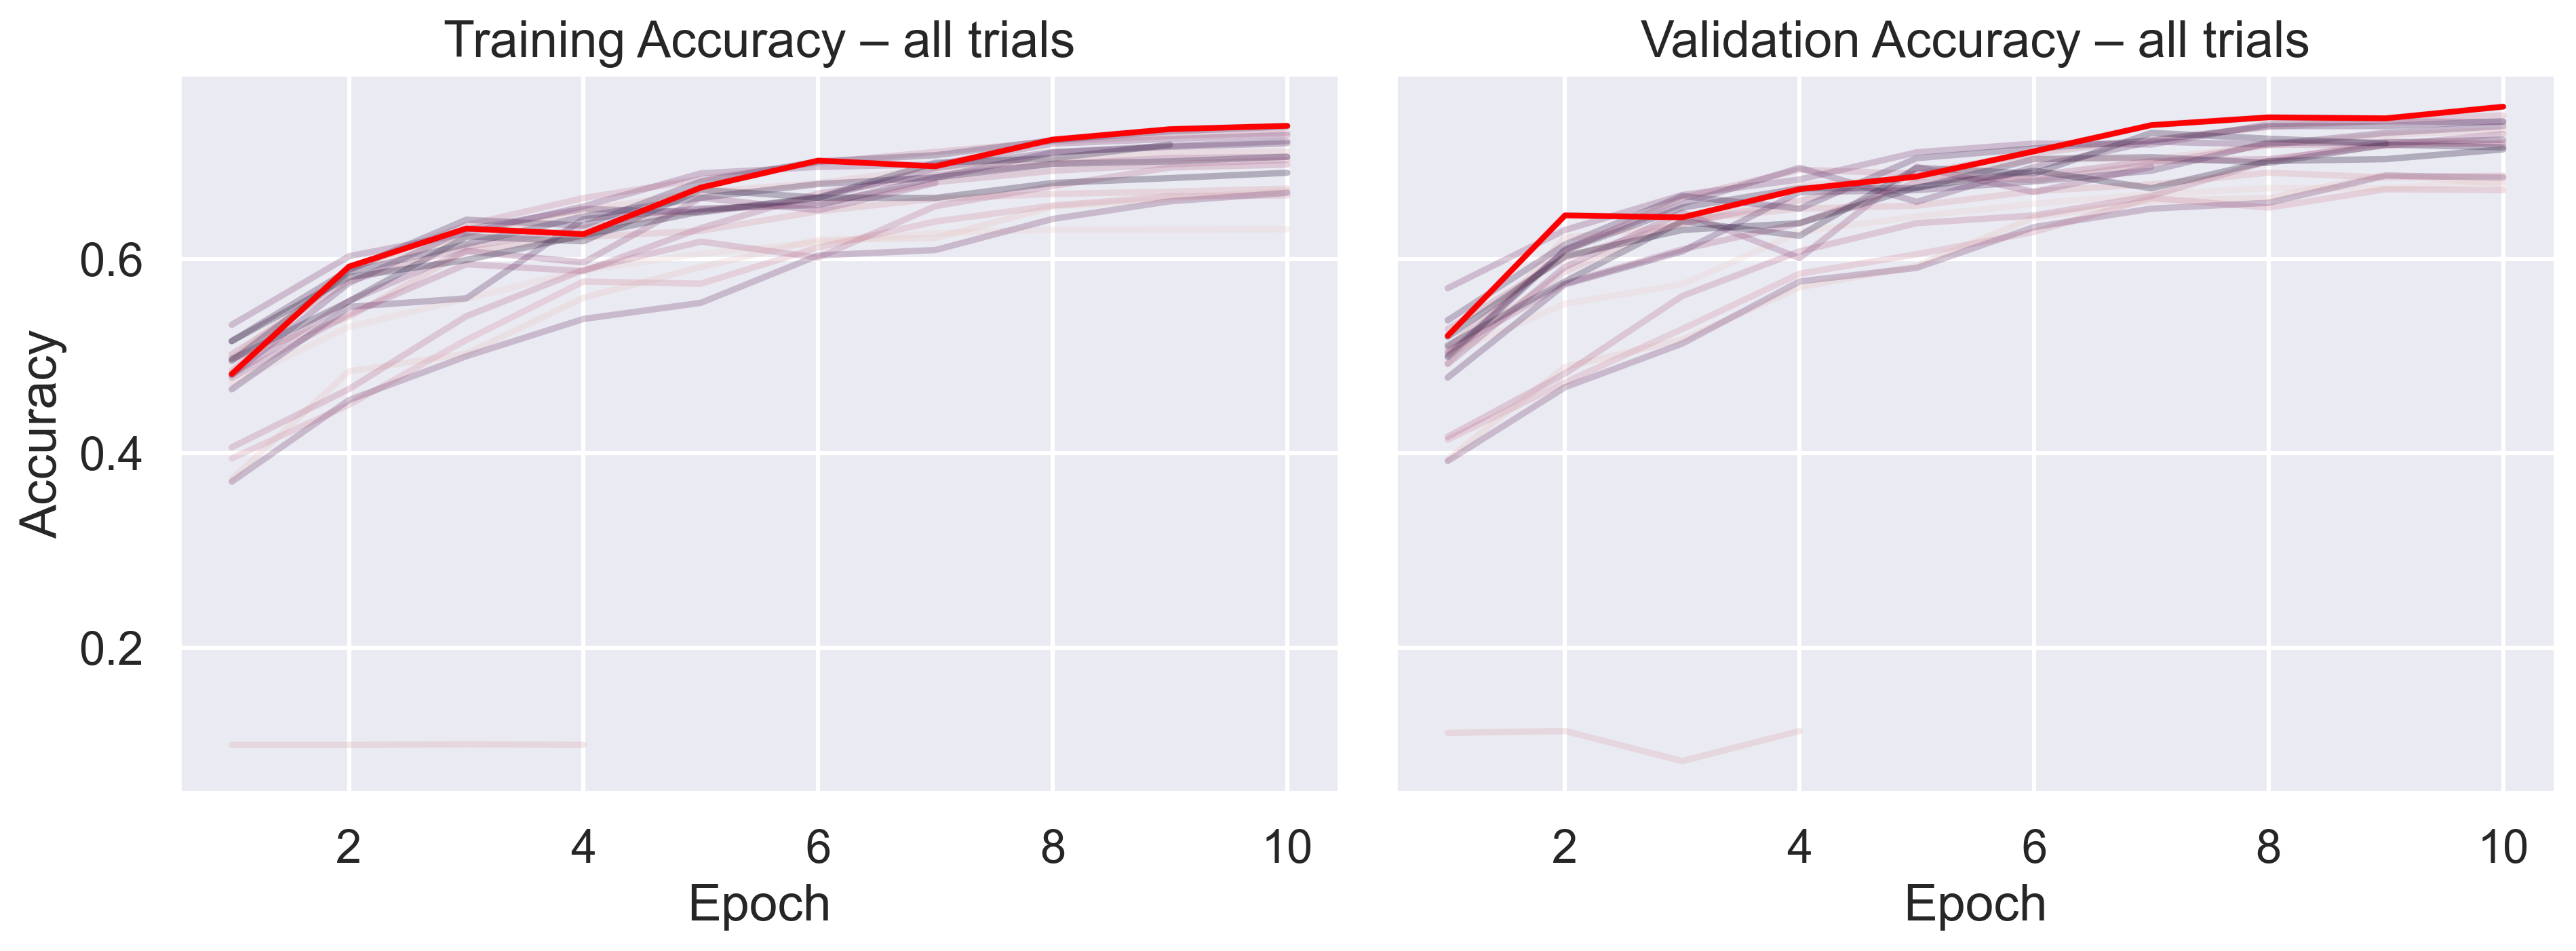
\includegraphics[width=\imagewidth, height=\imageheight, keepaspectratio]{all_trials_accuracy.png}
    \end{figure}
\end{frame}

%___________________________________________________________________

%___________________________________________________________________

\begin{frame}{Lernrate während des Trainings}
    \begin{figure}
        \centering
        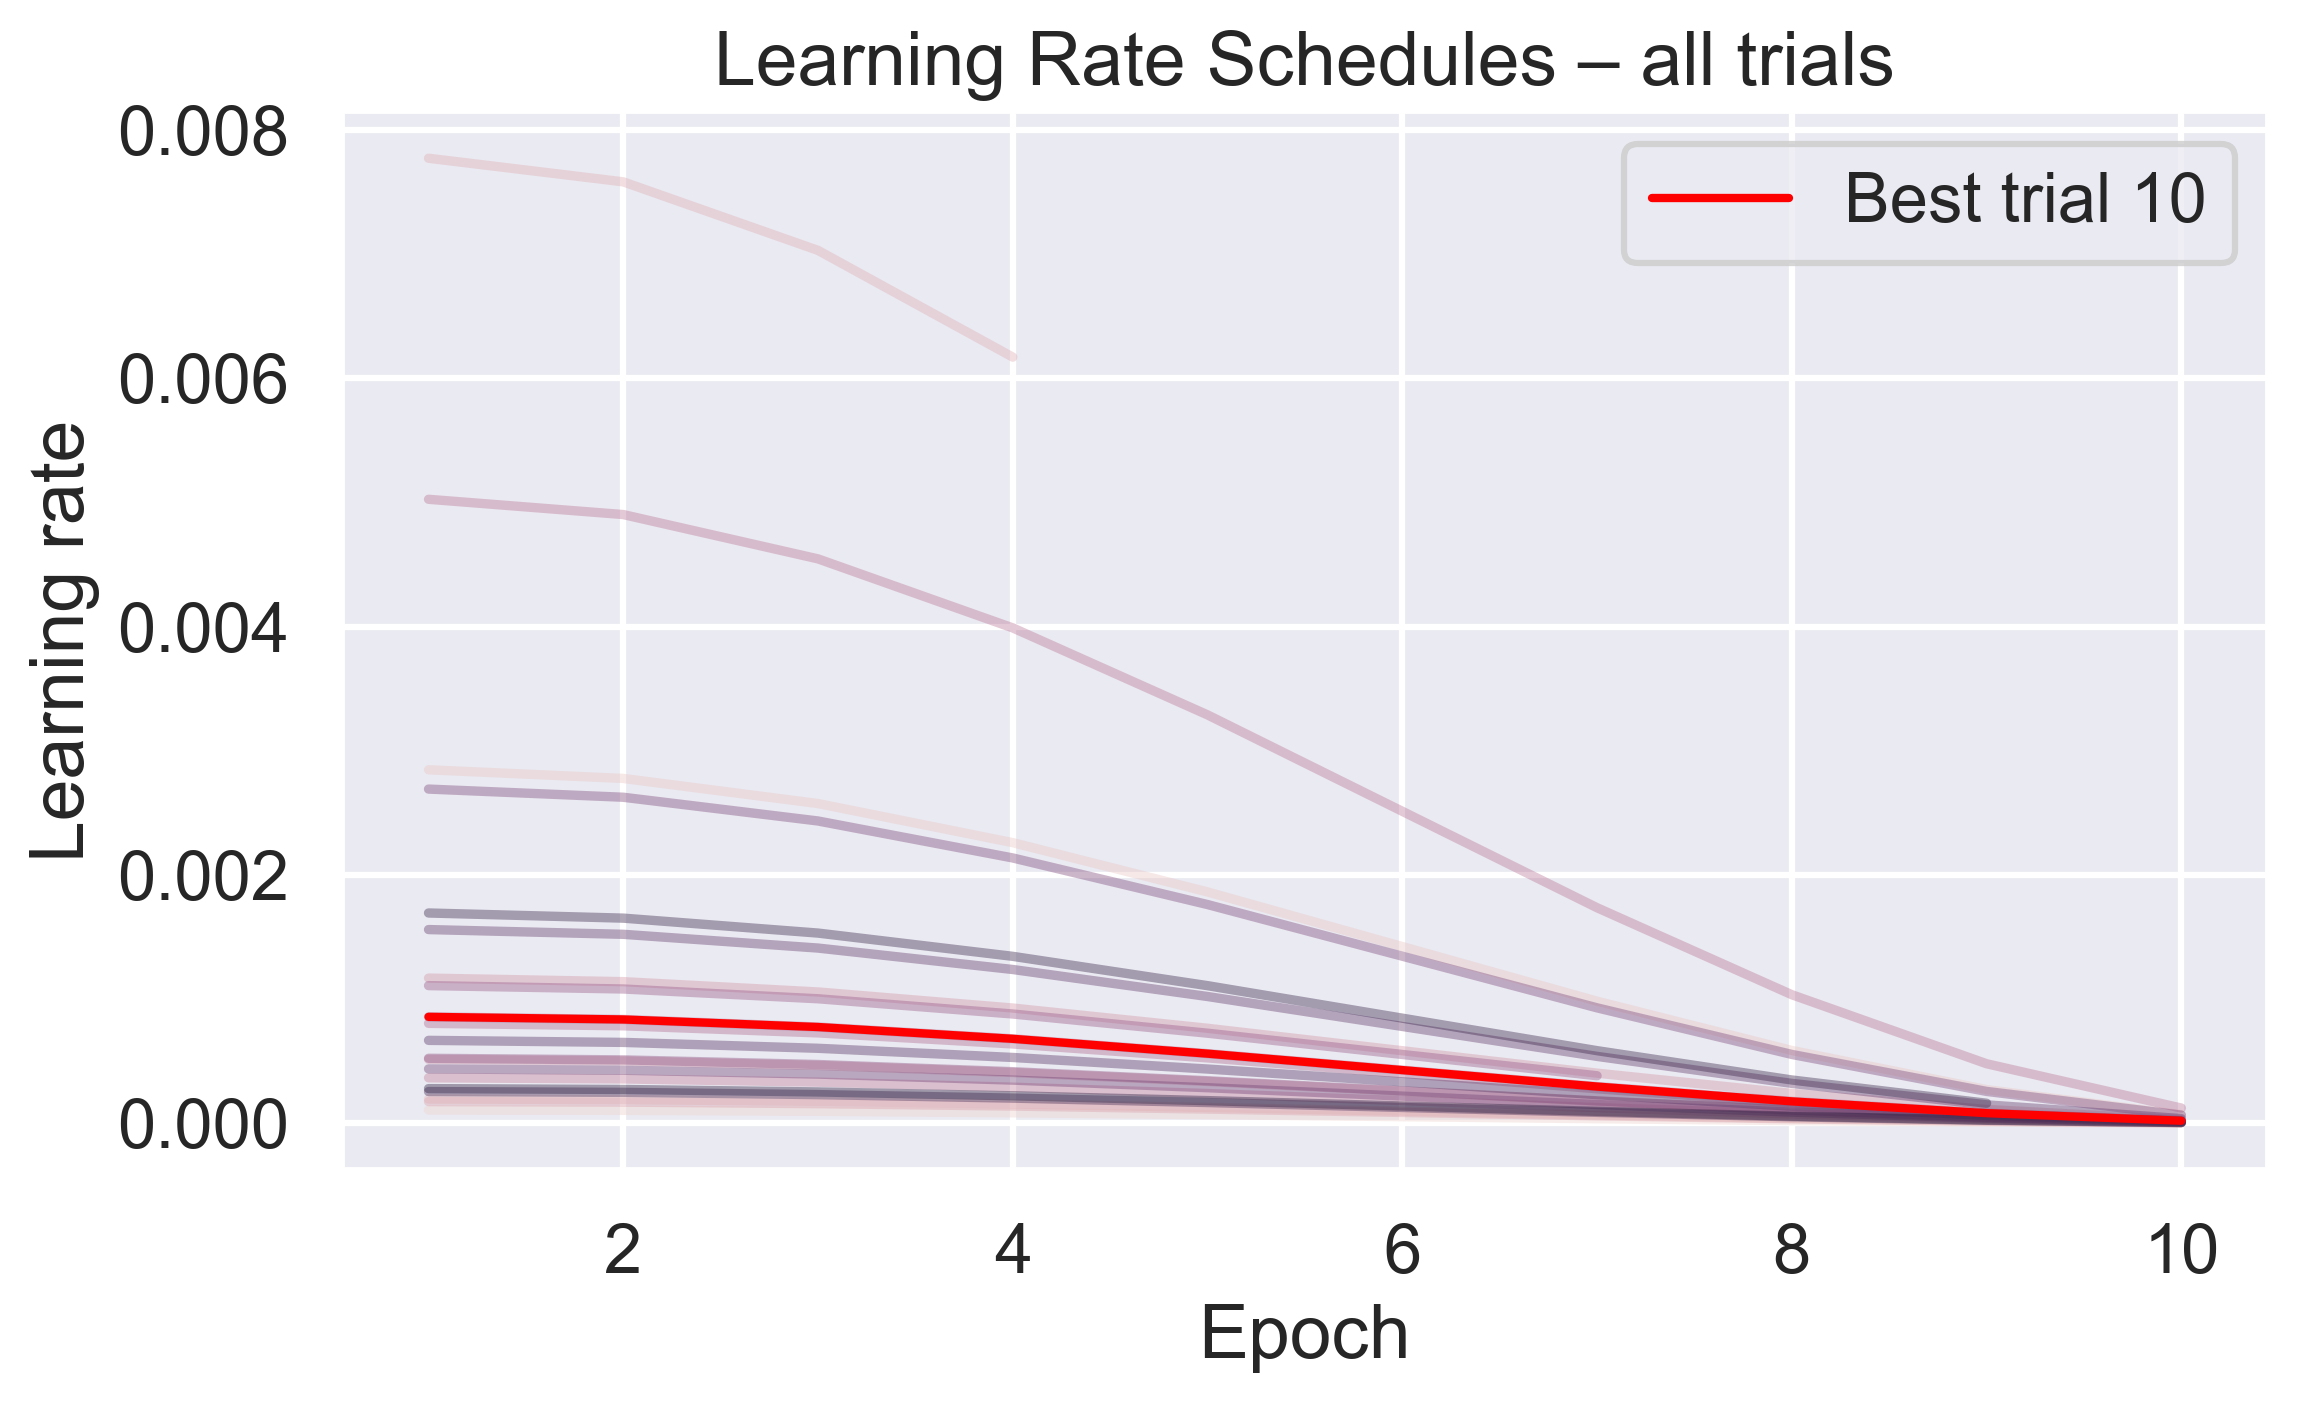
\includegraphics[width=\imagewidth, height=\imageheight, keepaspectratio]{all_trials_lr.png}
    \end{figure}
\end{frame}

\begin{frame}{Settings für das Training}
\textbf{Trainingsdaten:}
\begin{itemize}
    \item $N_{\text{train}} = 49\,000$
    \item Batchgröße: $256$ 
    \item Anzahl Worker für DataLoader: $12$ (hohe Parallelisierung)
\end{itemize}

\textbf{Training:}
\begin{itemize}
    \item Epochen: $10$ pro Runde
    \item Anzahl Trials (für Bayesian Search): $20$
    \item Iterationen pro Epoche: $\lceil 49000 / 256 \rceil \approx 192$
\end{itemize}

\textbf{Hardware:}
\begin{itemize}
    \item GPU: RTX 4060 Ti, 16 GB VRAM, 3D-Auslastung 100\%, RAM 40\%
    \item CPU: Ryzen 5 7600X, 12 Kerne, 100\% Auslastung
    \item Arbeitsspeicher: 32 GB DDR5, 100\% Auslastung
\end{itemize}

\textbf{Runtime:} abhängig von Batchgröße, Epochenzahl und Modell
\end{frame}

%___________________________________________________________________

\begin{frame}{Hardware Auslastung}
    \begin{figure}
        \centering
        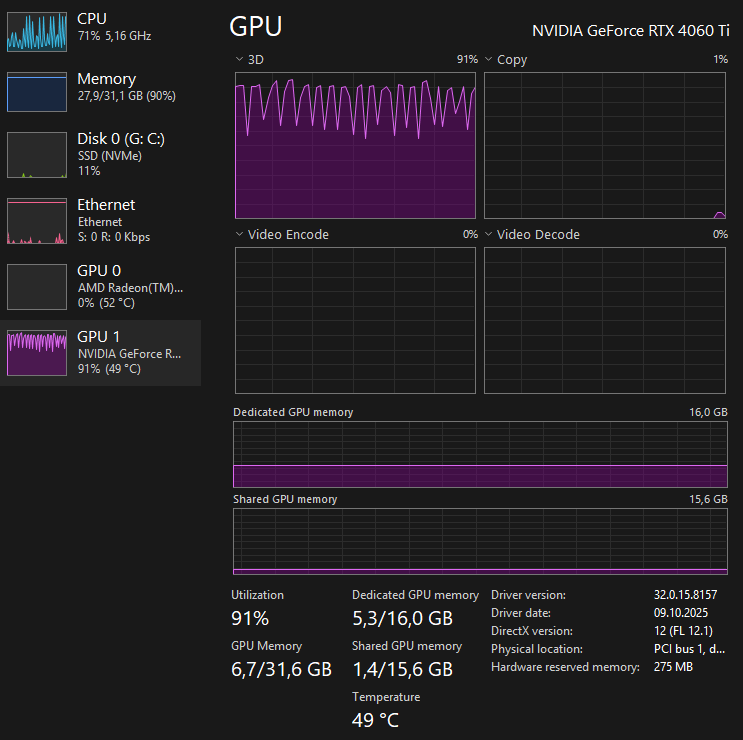
\includegraphics[width=\imagewidth, height=\imageheight, keepaspectratio]{machine.png}
    \end{figure}
\end{frame}

%___________________________________________________________________

\begin{frame}{Laufzeiten}
    \begin{figure}
        \centering
        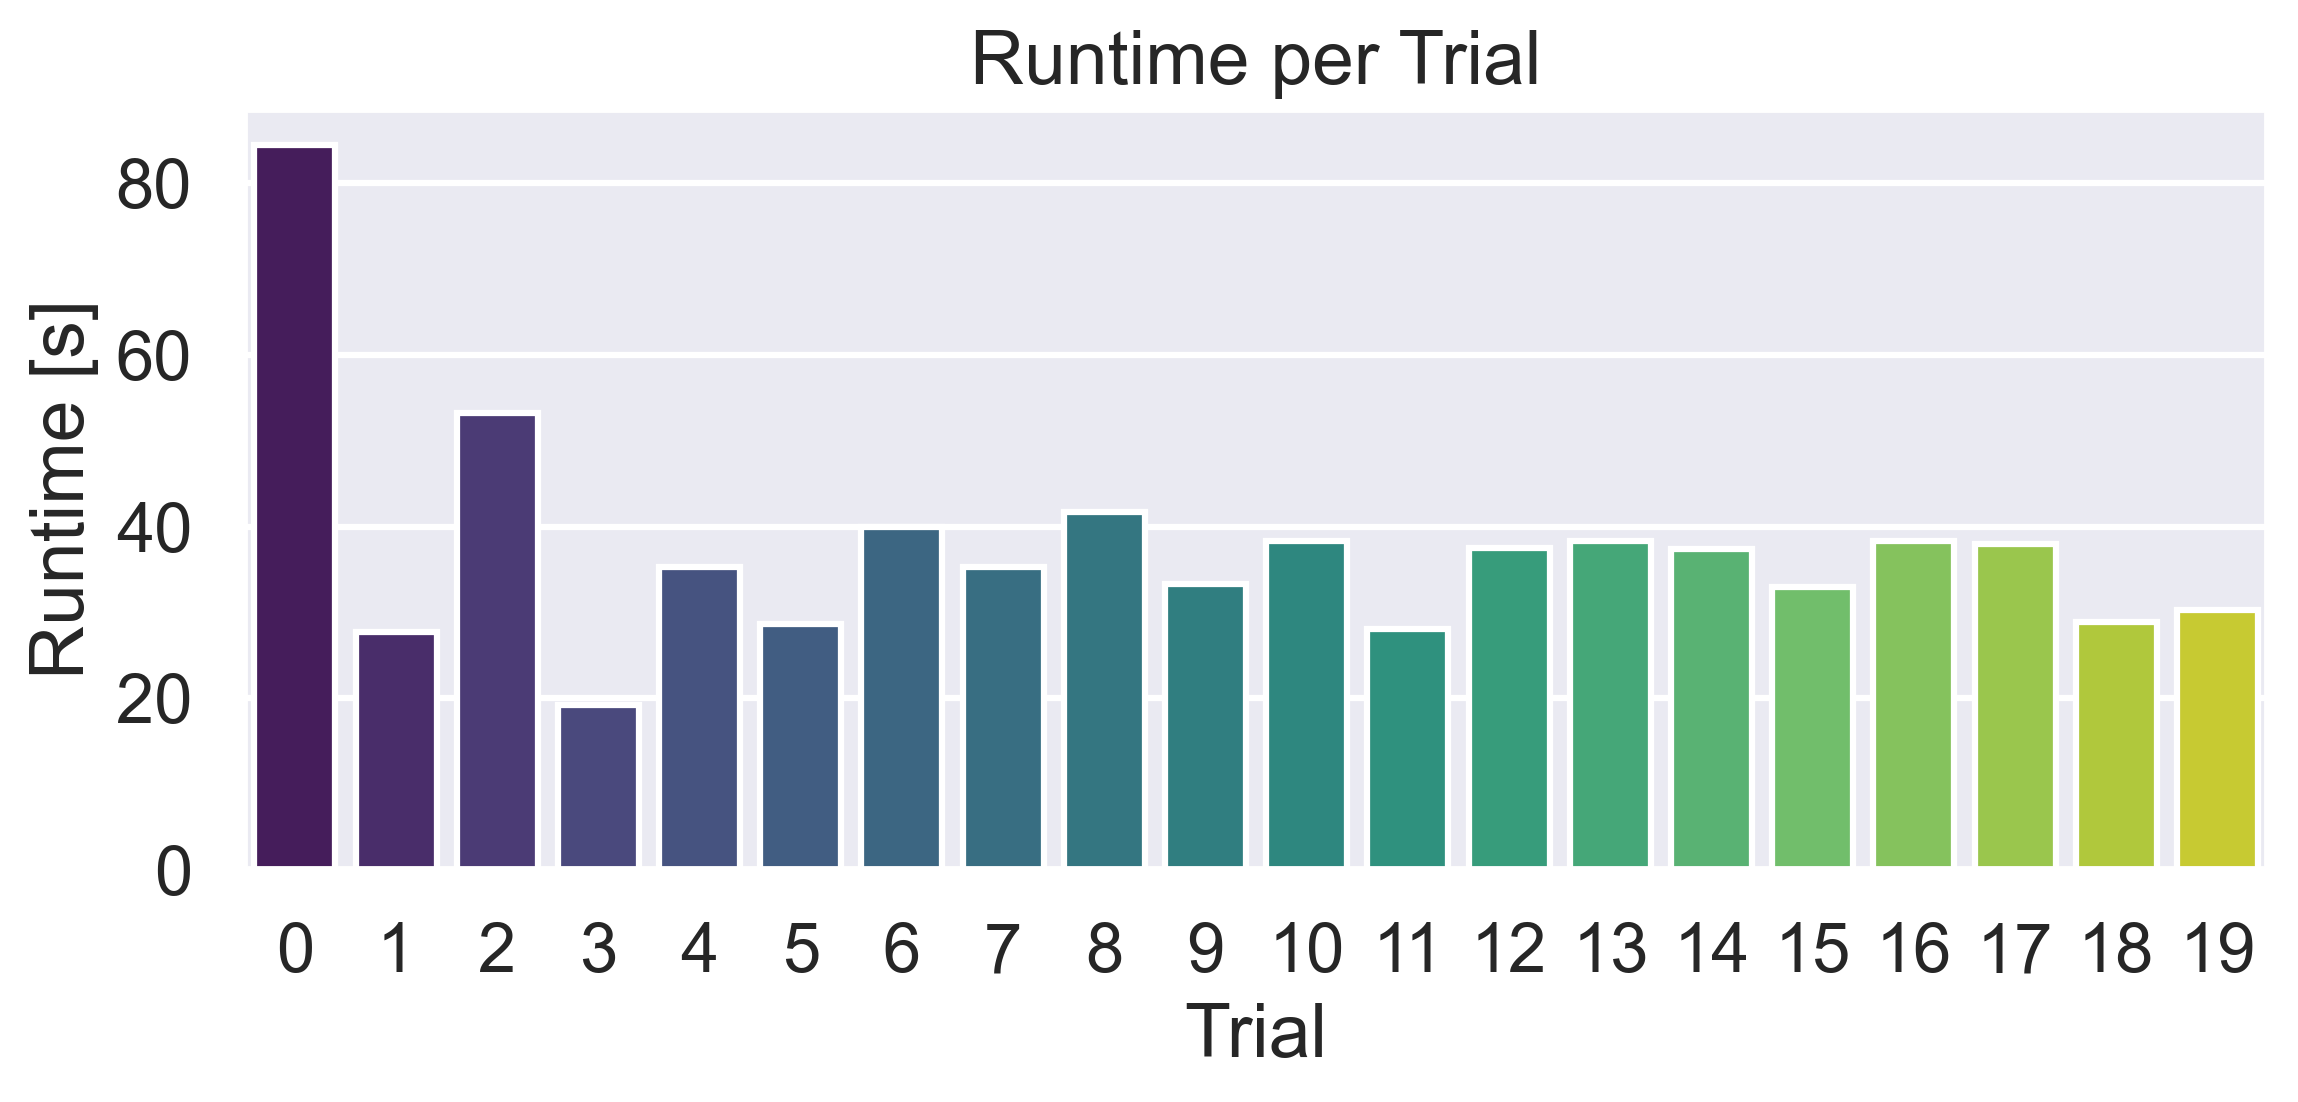
\includegraphics[width=\imagewidth, height=\imageheight, keepaspectratio]{runtime_per_trial.png}
    \end{figure}
\end{frame}

%___________________________________________________________________

\begin{frame}{Gradcam für Katze}
    \begin{figure}
        \centering
        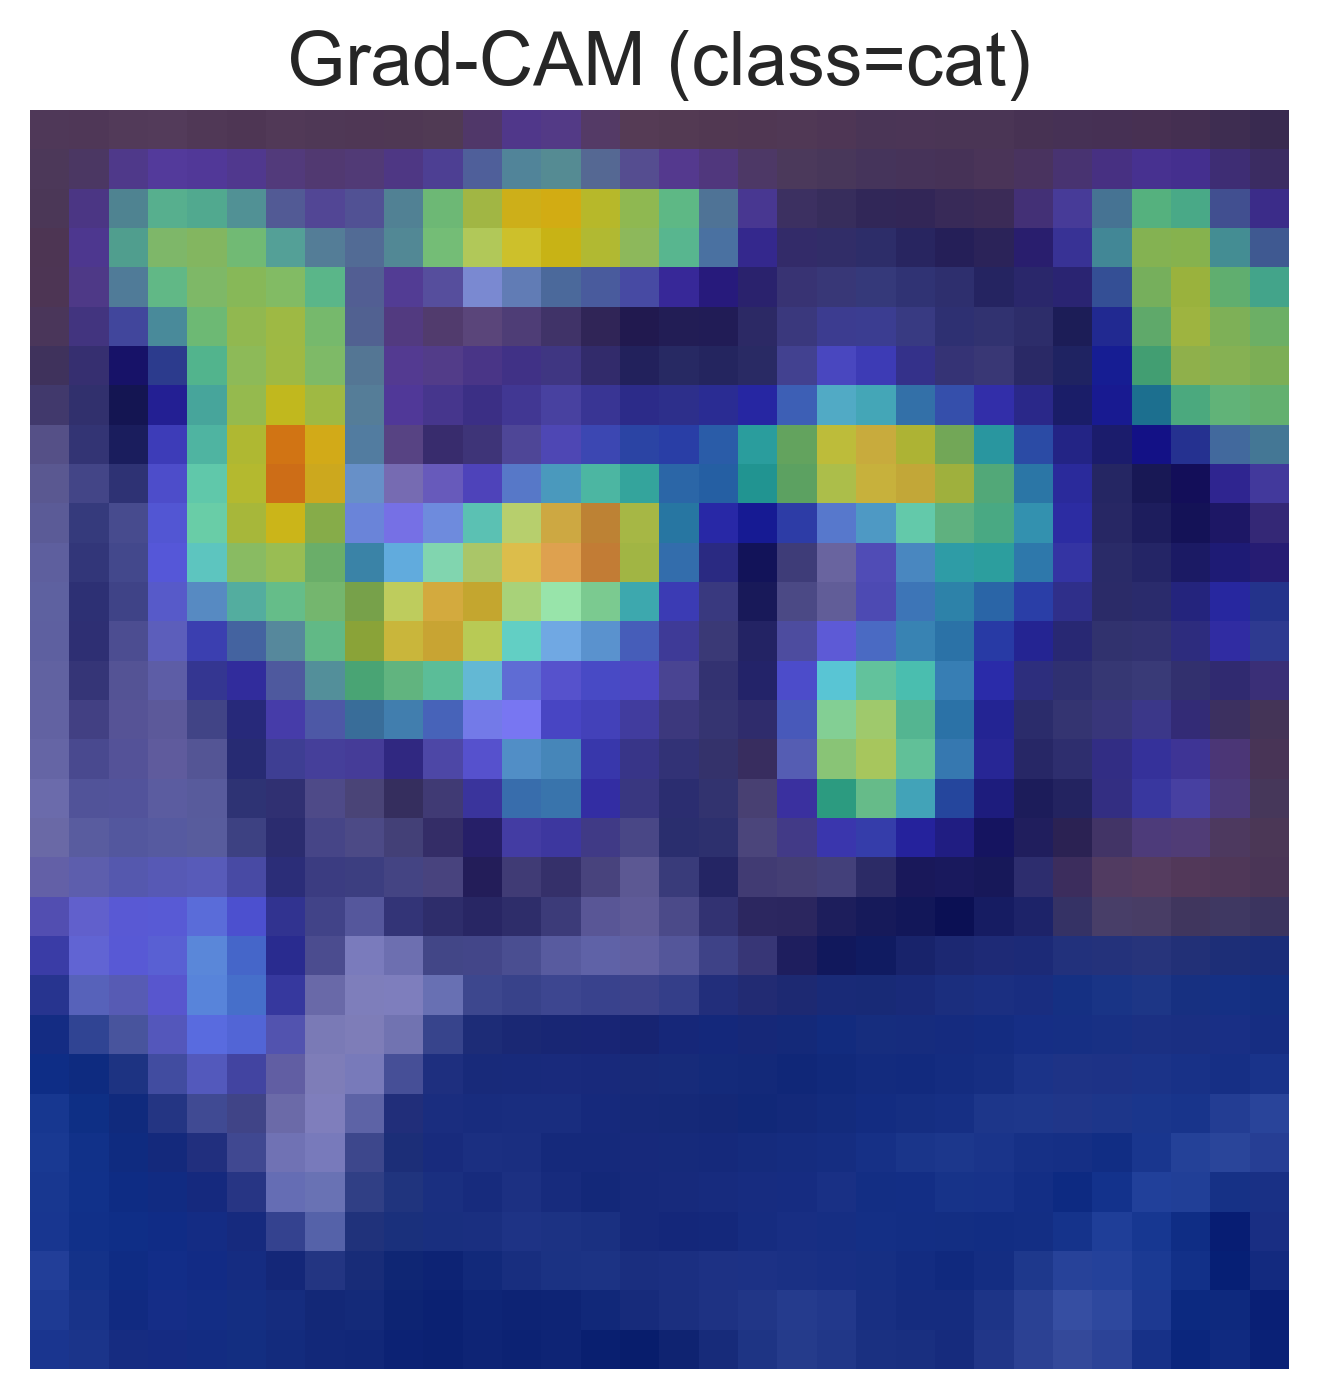
\includegraphics[width=\imagewidth, height=\imageheight, keepaspectratio]{gradcam.png}
    \end{figure}
\end{frame}


%___________________________________________________________________

\begin{frame}[fragile]{Early Stopping}
\textbf{Motivation:} 
\begin{itemize}
    \item Training kann zu lange laufen oder overfitten nach mehreren Epochen
    \item Stoppt Training, wenn keine Verbesserung der Validierungsgenauigkeit erfolgt
\end{itemize}

\textbf{Prinzip:}
\begin{itemize}
    \item Behalte besten Validierungswert
    \item Zähle Epochen ohne Verbesserung
    \item Stoppe, wenn \texttt{epochs\_no\_improve >= patience}
\end{itemize}

\textbf{Codebeispiel:}
\begin{verbatim}
if val_acc > best_val_acc:
    best_val_acc = val_acc
    epochs_no_improve = 0
else:
    epochs_no_improve += 1
    if epochs_no_improve >= patience:
        break
\end{verbatim}
\end{frame}
